\documentclass{article}

\usepackage[spanish]{babel}
\usepackage[utf8]{inputenc}
\usepackage[right=1.5cm,left=1.5cm,top=1.5cm,bottom=1.5cm]{geometry}

\title{Taller 3A\\ Estadística genómica}
\author{Juan David Henao Sánchez}

\usepackage{Sweave}
\begin{document}
\Sconcordance{concordance:JuanHenao_Taller3A.tex:JuanHenao_Taller3A.Rnw:%
1 9 1 1 0 9 1 1 2 1 0 1 1 3 0 2 2 1 0 1 1 5 0 1 1 19 0 2 2 5 0 2 2 1 0 %
2 1 11 0 2 1 3 0 2 2 1 0 1 1 7 0 2 2 20 0 2 2 1 0 2 1 19 0 2 2 5 0 2 2 %
1 0 1 1 5 0 1 1 11 0 1 2 2 1}


\maketitle

\section*{Sobre unos datos del GEO (una sola medición en el tiempo) que comparen dos condiciones, identifique los genes diferencialmente expresados usando acde:
}

\begin{itemize}
\item{Cargando las librerias}
\begin{Schunk}
\begin{Sinput}
> library(acde)
> library("DESeq")
\end{Sinput}
\end{Schunk}
\item{Cargando los datos}
\begin{Schunk}
\begin{Sinput}
> data <- read.table("GSE58972_RELA_6h_processed_data.txt", h=T)
> dim(data)
\end{Sinput}
\begin{Soutput}
[1] 23284     8
\end{Soutput}
\begin{Sinput}
> head(data)
\end{Sinput}
\begin{Soutput}
           gene description WT_6h_1 WT_6h_2 WT_6h_3 RELA_6h_1 RELA_6h_2
1 0610005C13Rik          na       9      12      12        11        16
2 0610007C21Rik          na     534     581     562       512       537
3 0610007L01Rik          na    2124    2197    2168      2811      2706
4 0610007N19Rik          na      17      26      21        18        20
5 0610007P08Rik          na    1410    1504    1543      1546      1577
6 0610007P14Rik          na    2049    2008    2074      2192      2192
  RELA_6h_3
1        10
2       501
3      2265
4        15
5      1353
6      1968
\end{Soutput}
\end{Schunk}
\item{Gráficando los datos cargados}
\begin{Schunk}
\begin{Sinput}
> boxplot(data[, 3:8], main="Boxplot Mus musculus", col="lightgreen", cex.names=0.2, las=2)
\end{Sinput}
\end{Schunk}
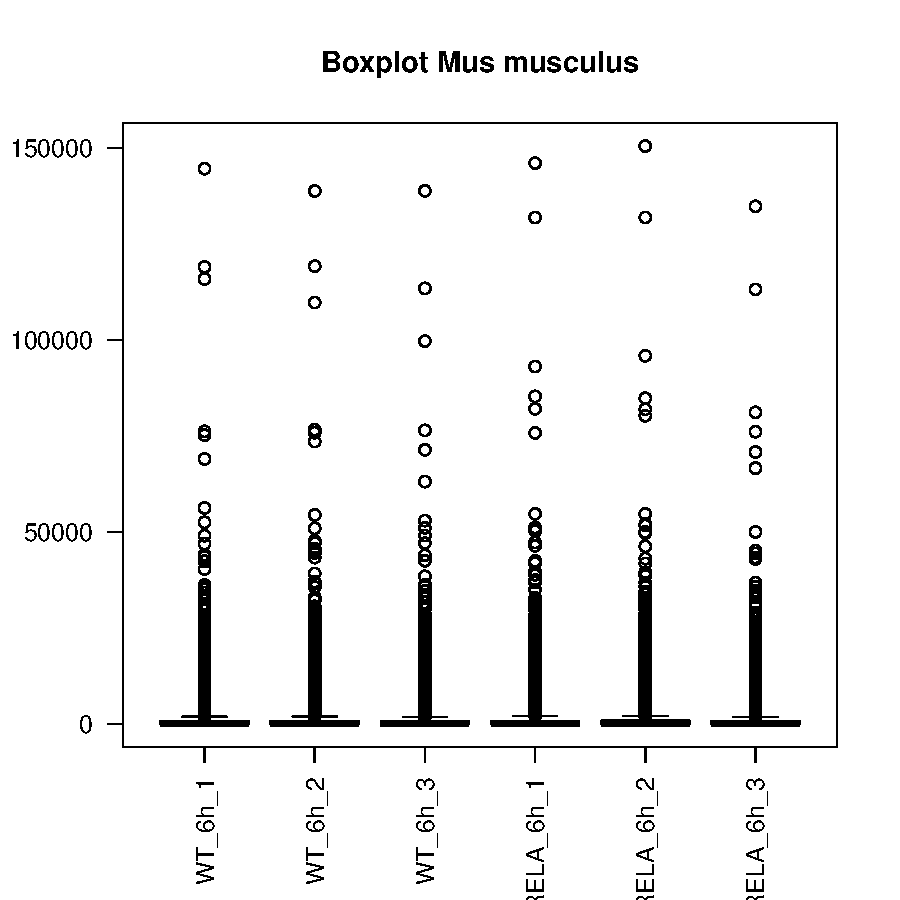
\includegraphics{JuanHenao_Taller3A-003}
\item{Creando el CountDataSet}
\begin{Schunk}
\begin{Sinput}
> rownames(data) <- data$gene
> countsTable <- data[,3:8]
> head(countsTable)
\end{Sinput}
\begin{Soutput}
              WT_6h_1 WT_6h_2 WT_6h_3 RELA_6h_1 RELA_6h_2 RELA_6h_3
0610005C13Rik       9      12      12        11        16        10
0610007C21Rik     534     581     562       512       537       501
0610007L01Rik    2124    2197    2168      2811      2706      2265
0610007N19Rik      17      26      21        18        20        15
0610007P08Rik    1410    1504    1543      1546      1577      1353
0610007P14Rik    2049    2008    2074      2192      2192      1968
\end{Soutput}
\begin{Sinput}
> conds <- factor( c( "WT", "WT", "WT", "treated","treated","treated"))
> cds <- newCountDataSet( countsTable, conds )
\end{Sinput}
\end{Schunk}
\item{Estimando el tamaño de los datos}
\begin{Schunk}
\begin{Sinput}
> cds <- estimateSizeFactors( cds )
> sizeFactors(cds)
\end{Sinput}
\begin{Soutput}
  WT_6h_1   WT_6h_2   WT_6h_3 RELA_6h_1 RELA_6h_2 RELA_6h_3 
0.9731925 0.9971984 0.9465783 1.0701892 1.0843975 0.9475568 
\end{Soutput}
\end{Schunk}
\item{Normalización}
\begin{Schunk}
\begin{Sinput}
> head(counts(cds,normalized=TRUE))
\end{Sinput}
\begin{Soutput}
                  WT_6h_1    WT_6h_2    WT_6h_3  RELA_6h_1  RELA_6h_2
0610005C13Rik    9.247913   12.03371   12.67724   10.27856   14.75474
0610007C21Rik  548.709529  582.63232  593.71741  478.42006  495.20587
0610007L01Rik 2182.507565 2203.17247 2290.35471 2626.63826 2495.39494
0610007N19Rik   17.468281   26.07305   22.18517   16.81946   18.44342
0610007P08Rik 1448.839768 1508.22549 1630.08179 1444.60432 1454.26379
0610007P14Rik 2105.441620 2013.64148 2191.04967 2048.23588 2021.39901
               RELA_6h_3
0610005C13Rik   10.55346
0610007C21Rik  528.72820
0610007L01Rik 2390.35804
0610007N19Rik   15.83019
0610007P08Rik 1427.88275
0610007P14Rik 2076.92037
\end{Soutput}
\end{Schunk}
\item{Estimando las diferencias}
\begin{Schunk}
\begin{Sinput}
> cds <- estimateDispersions( cds )
> res = nbinomTest(cds,"WT","treated")
> head(res)
\end{Sinput}
\begin{Soutput}
             id   baseMean  baseMeanA  baseMeanB foldChange log2FoldChange
1 0610005C13Rik   11.59094   11.31962   11.86225  1.0479369     0.06755185
2 0610007C21Rik  537.90223  575.01975  500.78471  0.8709000    -0.19942100
3 0610007L01Rik 2364.73767 2225.34492 2504.13042  1.1252774     0.17028074
4 0610007N19Rik   19.46993   21.90883   17.03102  0.7773587    -0.36334771
5 0610007P08Rik 1485.64965 1529.04902 1442.25029  0.9432335    -0.08431310
6 0610007P14Rik 2076.11467 2103.37759 2048.85175  0.9740770    -0.03789226
          pval        padj
1 0.9398718481 1.000000000
2 0.0067509416 0.078064572
3 0.0001904397 0.004043898
4 0.3435939599 0.876773371
5 0.1160588262 0.527125188
6 0.4241029562 0.939431937
\end{Soutput}
\end{Schunk}
\item{Gráficando los resultados obtenidos}
\begin{Schunk}
\begin{Sinput}
> plotMA(res)
\end{Sinput}
\end{Schunk}
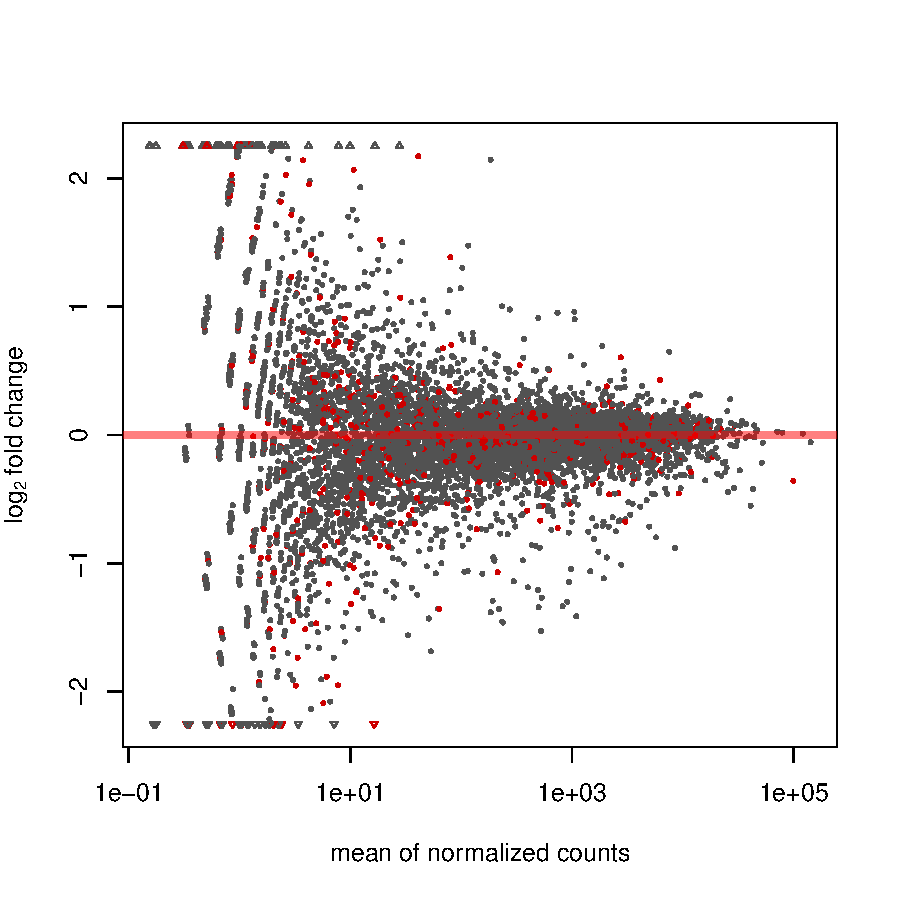
\includegraphics{JuanHenao_Taller3A-008}
\item{Resultados finales}
\begin{Schunk}
\begin{Sinput}
> resSig = res[ res$padj < 0.1, ]
> na.omit(dim(resSig))
\end{Sinput}
\begin{Soutput}
[1] 8364    8
\end{Soutput}
\begin{Sinput}
> na.omit(head(resSig))
\end{Sinput}
\begin{Soutput}
             id  baseMean baseMeanA baseMeanB foldChange log2FoldChange
2 0610007C21Rik  537.9022  575.0198  500.7847   0.870900     -0.1994210
3 0610007L01Rik 2364.7377 2225.3449 2504.1304   1.125277      0.1702807
          pval        padj
2 0.0067509416 0.078064572
3 0.0001904397 0.004043898
\end{Soutput}
\end{Schunk}
\end{itemize}
\end{document}

